\frame{

\begin{enumerate}
\setcounter{enumi}{1}
 \item Marco teórico y conceptual
  \begin{itemize}
    \item Contratación Pública y \eproc.
    \item Web Semántica.
    \item \linkeddata y \opendata.
     \item \eproc y Semántica.
  \end{itemize}

\end{enumerate}

}


\subsection*{Contratación Pública Electrónica}
\frame{
  \frametitle{\eproc}
 \begin{itemize}
        \item Sector estratégico. $17$\%  del PIB.
        \item Impulsado desde la Unión Europea (adopción paulatina). \linebreak Plan de Acción 2004 y Europa 2020.
        \item Múltiples fases y etapas (maraña de requisitos técnicos).
        \item Información y datos valiosos. Sociedad de la Información.
        \item Marco legal definido y en evolución (homogeneización).
	\item 16K anuncios de licitación nuevos al día.
        \item Necesidad de impulso de la participación de las pequeñas y medianas empresas (PYMES).
\end{itemize}

}

\frame{
  \frametitle{Fases de \eproc} 

\begin{figure}[htb]
\centering
	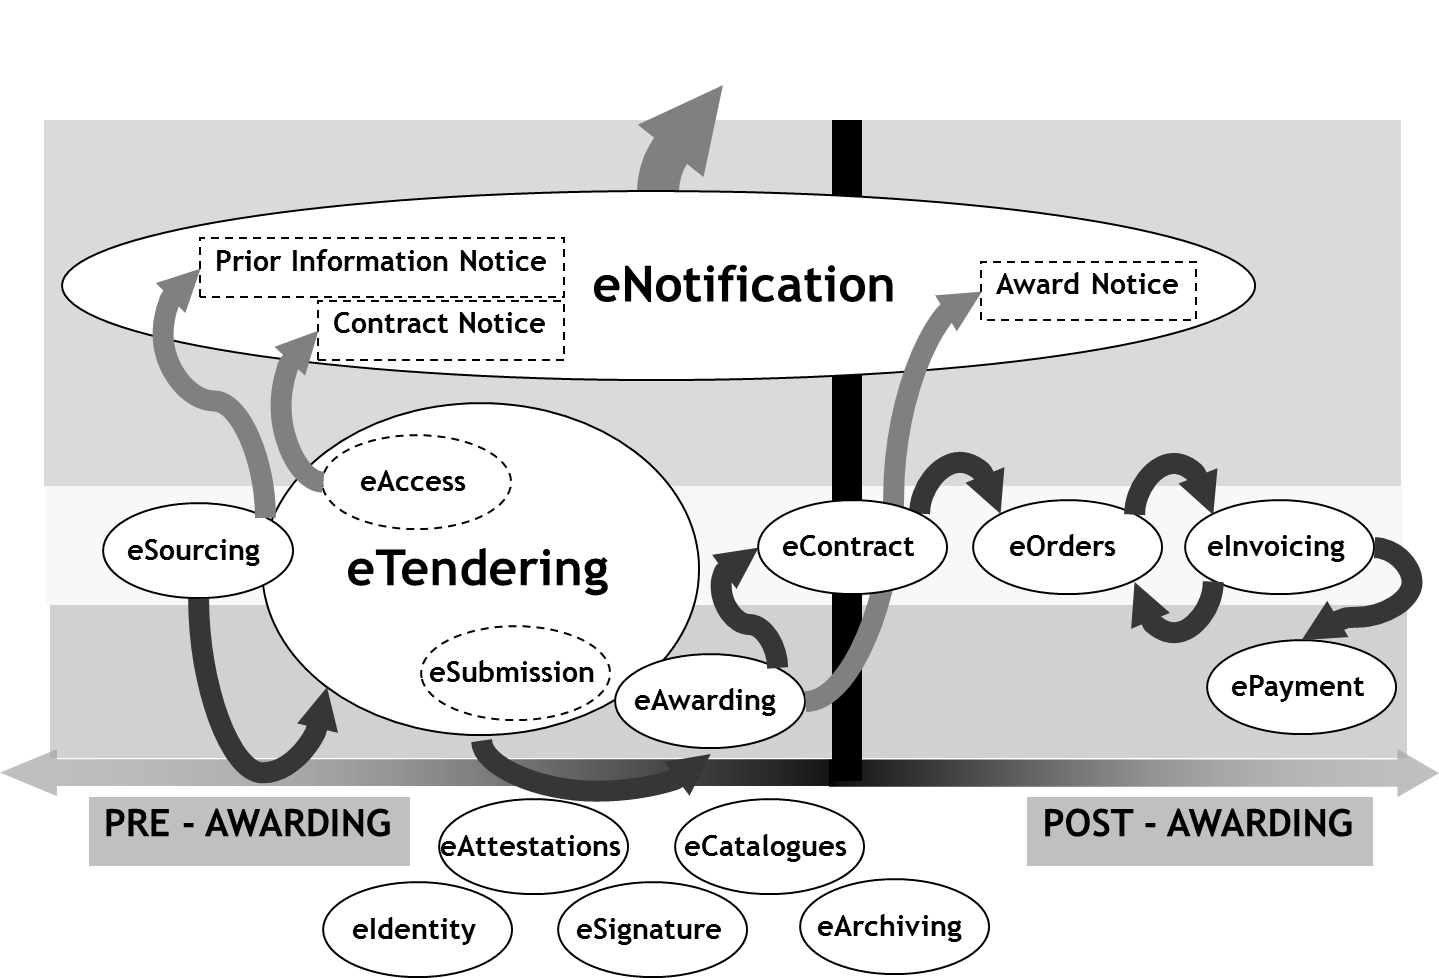
\includegraphics[width=8cm]{imgs/e-proc-complexity}
\caption{Diagrama de Complejidad y Fases de e-Procurement.}
\end{figure}
{\tiny Fuente: Unión Europea.}
}

\frame{
  \frametitle{Definición de \eproc} 

\begin{exampleblock}{Contratación Pública Electrónica}<1->
 La contratación electrónica es un término general utilizado para designar la sustitución de los
procedimientos basados en soporte de papel por el tratamiento y la comunicación mediante
TIC a lo largo de toda la cadena de contratación pública. 
\end{exampleblock}
\begin{itemize}[<2->]
 \item Publicación de los anuncios de licitación.
 \item Suministro del pliego de condiciones.
 \item Presentación de ofertas.
 \item Adjudicación.
 \item Facturación y pago.
 \item \ldots
\end{itemize}

}


\frame{
  \frametitle{Silos de Información} 

\begin{figure}[htb]
\centering
 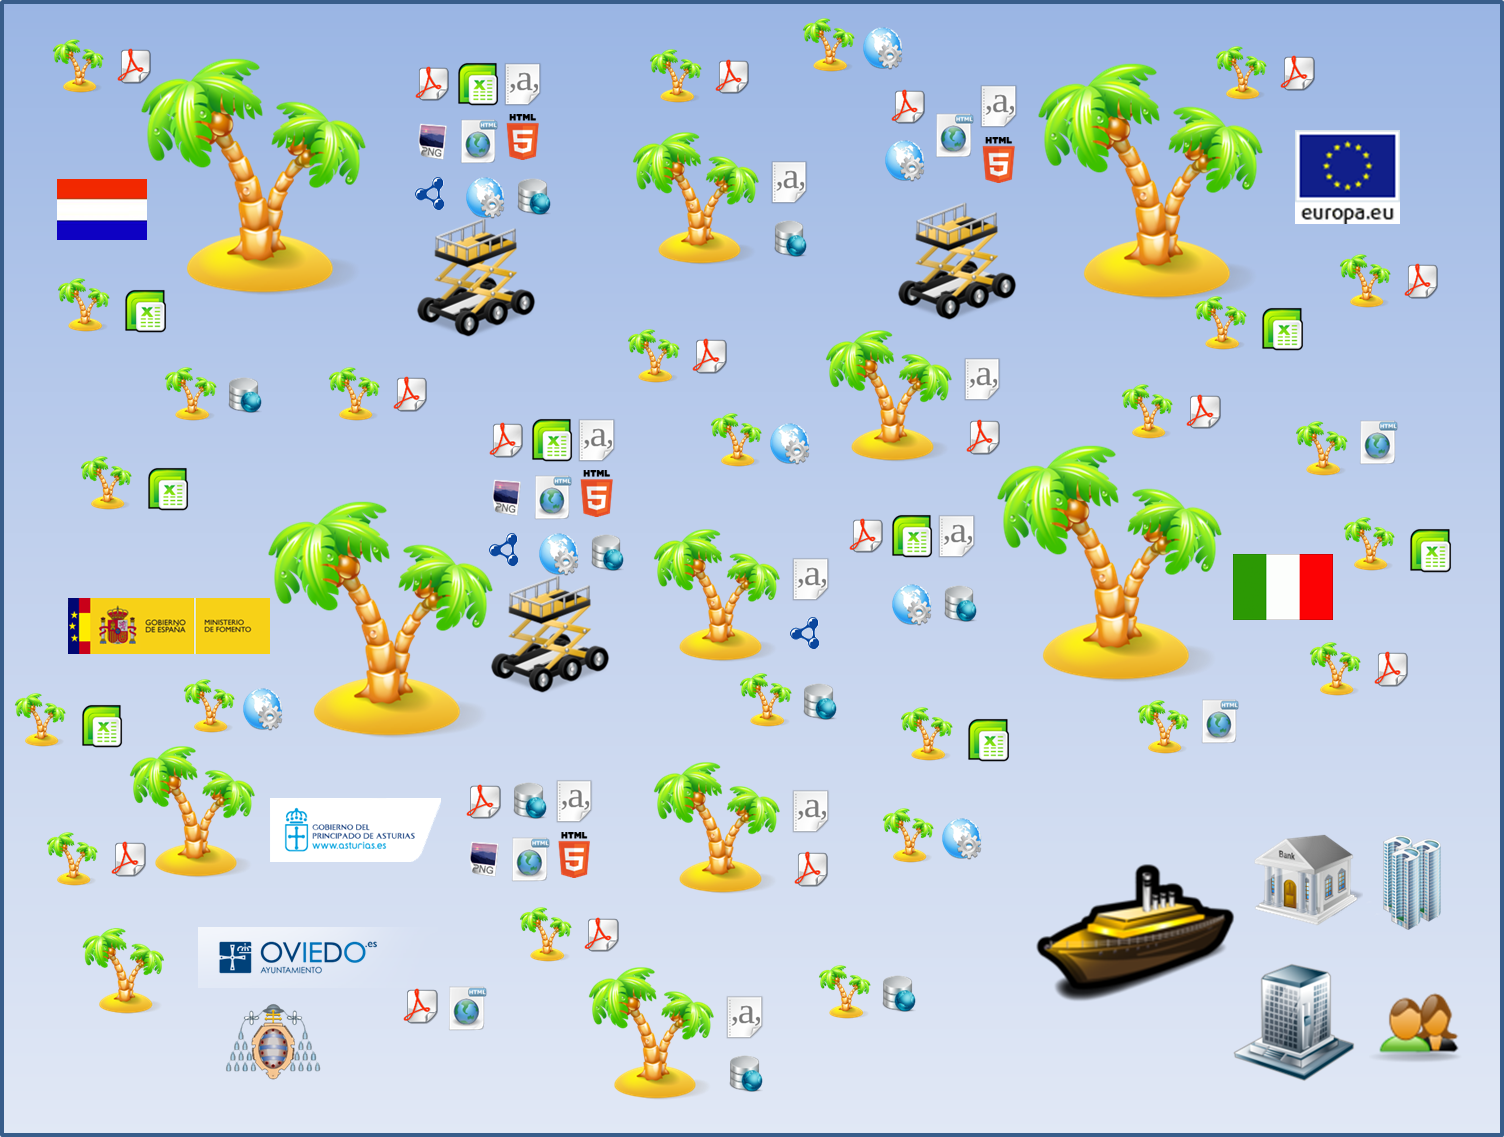
\includegraphics[width=8cm]{imgs/maremagnum}
\caption{Silos de Información en \eproc de la Unión Europea.}
\end{figure}
}


\frame{
  \frametitle{Multiling\"{u}ismo y multiculturalidad.} 

\begin{figure}[htb]
\centering
 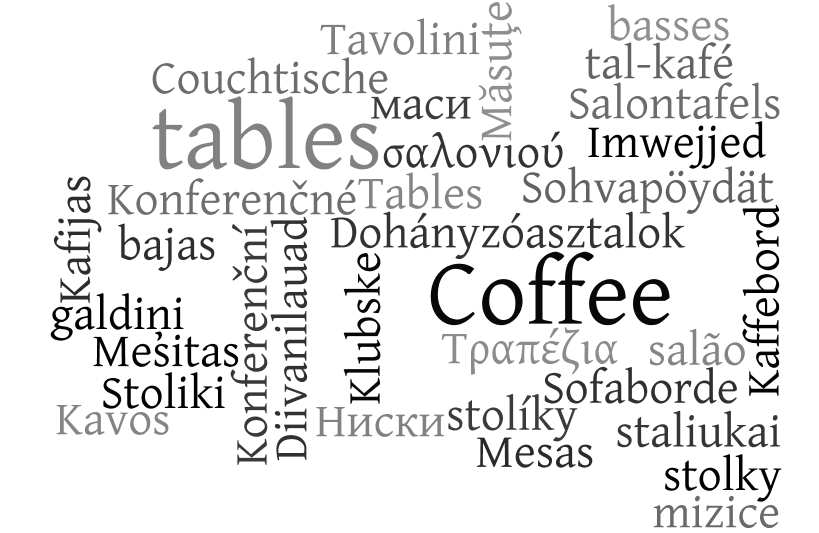
\includegraphics[width=8cm]{imgs/multilingue}
\caption{Concepto ``mesitas'', ``mesas de café'', etc.}
\end{figure}
}


\frame{
  \frametitle{Acciones de la Unión Europea} 

\begin{itemize}[<1->]
\item \textit{Tenders Electronic Daily} (TED) y Sistema de Información para la contratación pública europea (SIMAP).
\item Clasificaciones Estándar de Productos y Servicios (CPV).
\item Clasificación de regiones (NUTS).
\item Plataformas de Contratación.
\item Proyectos destacados:
\begin{enumerate}[<2->]
 \item \textbf{e-Certis}.
 \item \textbf{Fiscalis 2013}.
 \item \textbf{ePRIOR}.
 \item \textbf{PEPPOL}-\textit{Pan-European Public Procurement Online}.
 \item \textbf{STORK} -\textit{Secure idenTity acrOss euRope linKed}.
\end{enumerate}
\end{itemize}

}

\frame{
  \frametitle{\textit{Common Procurement Vocabulary}-CPV} 
\begin{figure}[htb]
\centering
	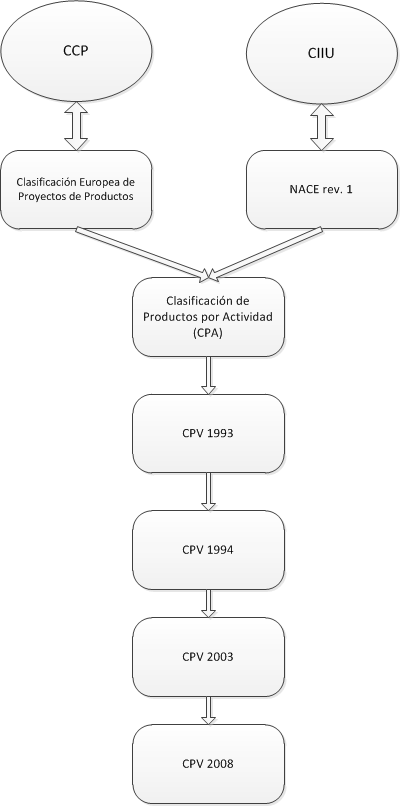
\includegraphics[width=3cm]{imgs/evo-cpv}
\caption{Evolución del \textit{Common Procurement Vocabulary}.}
\end{figure}

}


\frame{
  \frametitle{Modelo de Información} 

\begin{itemize}[<1->]
\item TED (XML-Schema).
\item CODICE (XML-Schema).
\item opXML (XML-Schema).
\item \ldots
\end{itemize}

\begin{block}{Valoración}<2->
 \begin{itemize}
\item Sobre-especificación.
\item Escasa convergencia (nombrado, especificidad, etc.) e interoperabilidad.
\item Falta de consenso.
\item Replicación de esfuerzos.
\item Necesidades transversales: publicación de información, gestión de pagos, etc.
\end{itemize}
\end{block}
}

\frame{
  \frametitle{Principales Problemas} 

\begin{alertblock}{Puntos de Mejora}<1->

\begin{itemize}
\item Dispersión de la información.
\item Mismo anuncio en más de una fuente.
\item Heterogeneidad de los formatos de los anuncios.
\item Diversidad de formatos de explotación.
\item Multiling\"{u}ismo y multiculturalidad.
\item Otros: almacenamiento, etc.
\end{itemize}

\end{alertblock}


}


\subsection*{Web Semántica}

\frame{
  \frametitle{Web Semántica}

\begin{block}{Características Principales}
 \begin{itemize}
\item Modelo de datos estándar para representar recursos. Grafo RDF (sujeto, predicado, objeto).
\item Formalización del conocimiento mediante ontologías basadas en lógica (\textit{DL}).
\item Facilidad para su extensión y crecimiento dinámico.
\item Aplicación de estándares en representación (OWL2) y acceso (SPARQL).
\item Baja intrusividad con sistemas existentes.
\item Mejora de la interoperabilidad e integración.
\item Soporte para la creación de sistemas basados en conocimiento.
\item Gran variedad de vocabularios, conjuntos de datos, etc., en distintos dominios.
\end{itemize}
\end{block}

}

\subsection*{Datos Enlazados}

\frame{
  \frametitle{\linkeddata}

\begin{columns}[c] % the "c" option specifies center vertical alignment
\column{.5\textwidth} % column designated by a command


\begin{block}{Principios}
 \begin{enumerate}
\item \textit{Use URIs as names for things.}
\item \textit{When someone looks up a URI, provide useful information, using the standards (RDF*, SPARQL).}
\item \textit{Include links to other URIs.}
\item \textit{Use HTTP URIs.}
\end{enumerate}
\end{block}


\column{.5\textwidth}

% 
%  \begin{itemize}
% \item $\star$-Disponible en la web en cualquier formato con una licencia abierta. Ej: imagen.
% \item $\star\star$-Disponible en la web con un formato de datos estructurado. Ej: MSExcel.
% \item $\star\star\star$-\ldots formato abierto. Ej: CSV.
% \item $\star\star\star\star$-\ldots basado en estándares W3C como RDF, SPARQL, etc.
% \item $\star\star\star\star\star$-\ldots enlazado a otros conjuntos de datos.
% \end{itemize}
% \end{exampleblock}

\begin{figure}[htb]
\centering
	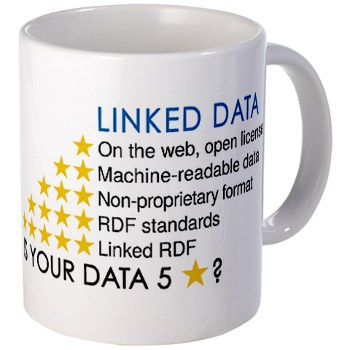
\includegraphics[width=3cm]{imgs/datosenlazados1}
\caption{Modelo $5\star$ (W3C).}
\end{figure}

\end{columns}

}

\frame{
  \frametitle{\linkeddata}

\begin{exampleblock}{Ventajas}
 \begin{itemize}
\item Realización práctica de la Web Semántica.
\item Identificación única, uso de HTTP URIs.
\item Modelo y acceso estándar.
\item Enriquecimiento de recursos, creación de enlaces.
\item Estructuración, modelo estándar RDF.
\item Expresividad, vocabularios y \datasets.
\item Reutilización de información y datos.
\item \ldots
\end{itemize}
\end{exampleblock}

}



\subsection*{Datos Abiertos}

\frame{
  \frametitle{\opendata}

\begin{block}{Los 8 principios}
 \begin{itemize}
\item Data Must Be \textbf{Complete}.
\item \ldots \textbf{Primary}.
\item \ldots \textbf{Timely}.
\item \ldots \textbf{Accessible}.
\item \ldots \textbf{Machine processable}.
\item Access Must Be \textbf{Non-Discriminatory}.
\item Data Formats Must Be \textbf{Non-Proprietary}.
\item Data Must Be \textbf{License-free}.
\end{itemize}
\end{block}
}


\frame{
  \frametitle{\opendata}

\begin{exampleblock}{Ventajas}
 \begin{itemize}
\item Inclusión.
\item Transparencia.
\item Responsabilidad.
\item Reutilización de información del sector público (PSI).
\item Generación de múltiples vistas de los datos.
\item Creación de servicios de valor añadido.
\item Integración de fuentes de datos.
\end{itemize}
\end{exampleblock}

}

\frame{
  \frametitle{Iniciativas \opendata} 

\begin{figure}[htb]
\centering
	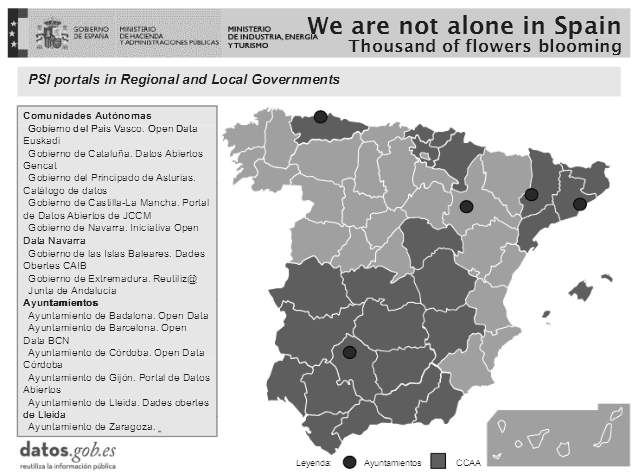
\includegraphics[width=7cm]{imgs/open-data-spain}
\caption{Datos Abiertos en España.}
\end{figure}
{\tiny Fuente: \url{http://datos.gob.es}}
}


\subsection*{Datos Abiertos Enlazados}

\frame{
  \frametitle{\lod}

\begin{figure}[htb]
\centering
	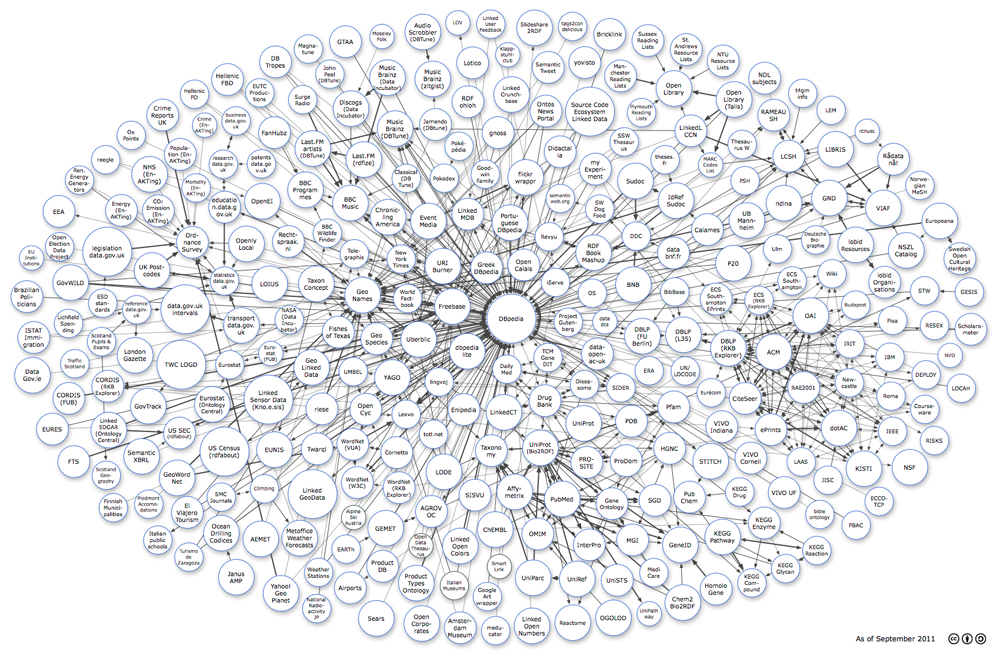
\includegraphics[width=4cm]{imgs/lod-cloud}
\caption{\lod \textit{cloud}.}
\end{figure}
\begin{itemize}
\item $203$ \datasets, $25$ billones de tripletas RDF y unos $395$ millones  de enlaces entre los datos (Sept. 2010).
\item Dominios: \textit{Media, Geographic, Government ($42.09$ \%), Publications, Cross-domain, Life sciences, etc.} (Ago. 2011).
\item $393$ \datasets (Jun. 2012).
\end{itemize}
{\tiny Fuente: R. Cyganiak \& A. Jentzsch.}
}

\frame{
  \frametitle{Web Semántica, \linkeddata, \opendata y \lod}

\begin{exampleblock}{Casos de Uso de éxito}
 \begin{itemize}
\item Soporte a la decisión médica.
\item Sugerencia de recursos turísticos.
\item Integración de aplicaciones.
\item Búsqueda semántica.
\item Gestión documental.
\item Información geográfica.
\item \ldots
\end{itemize}
\end{exampleblock}

}

\frame{
  \frametitle{Necesidades en \linkeddata}

 \begin{itemize}
\item ¿Qué datos se deben abrir, enlazar y publicar?.
\item ¿Cómo se deben producir los datos enlazados? ¿Cuál es el grado de cumplimiento de los principios?.
\item ¿Cuáles son los pasos/tareas de ejecución?.
\item ¿Qué buenas prácticas existen? ¿Validación, calidad, procedencia?.
\item ¿Cómo se facilita el consumo?.
\end{itemize}

}

\frame{
  \frametitle{Ciclos de Vida en \linkeddata}

\begin{itemize}
 \item \textit{Linked Data Design Considerations} [1].
 \item \textit{Linked Data Patterns} [2].
  \item Grupo de trabajo del W3C-\textit{Government Linked Data} (GLD) [3]:
  \begin{enumerate}
   \item \textit{Publishing Open Government Data} [4] y \textit{Best Practices} [5,6].
   \item \textit{Government Linked Data-Life Cycle} y \textit{Linked Data Cookbook} [7].
  \end{enumerate}
 \item \textit{LOD2 Stack} [8], proyecto europeo \textit{LOD2}.
 \item \textit{Toward a Basic Profile for Linked Data} [9], IBM y W3C.
 \item Metodología BCN y UNIOVI [10].
 \item \textit{Linked Open Data: The Essentials} [11].
 \item Otros: por país (UK, EEUU, etc.), empresa (\textit{Talis Platform}, TopQuadrant, etc.), etc.
\end{itemize}
}

\frame{
  \frametitle{Ciclos de Vida en \linkeddata}
\begin{alertblock}{Problemas encontrados}
 \begin{itemize}
\item Maremágnum recetas/metodologías/buenas prácticas.
\item Diferentes niveles de abstracción y mezcla en las tareas.
\item Baja definición de responsables en las tareas.
\item Baja especificación de resultados de las tareas.
\item Ajuste a casuística concreta.
\item Especificaciones teóricas o en desarrollo.
\item Ausencia de relación entre las mismas.
\item \ldots
\end{itemize}
\end{alertblock}
}


\subsection*{Contración Pública Electrónica y Semántica}
\frame{
  \frametitle{\eproc y Semántica}
\begin{block}{Actividades e Iniciativas}
 \begin{itemize}
\item Taxonomías de productos y servicios: CPA, CPC, CPV, NAICS, etc.
\item Vocabularios XML de negocio: ebXML, XBRL, SBVR o SCOR.
\item Vocabularios basados en semántica: \textit{GoodRelations}, \textit{ProductOntology}, \textit{Organizations ontology}, FOAF, etc.
\item Ontologías: República Checa y proyecto LOTED.
\item Proyectos europeos: LOD2 (WP9), LATC, PlanetData, etc.
\end{itemize}
\end{block}

}


\subsection*{Resumen}
\frame{
  \frametitle{Puntos Clave}
\begin{block}{...a considerar...}<1->
 \begin{itemize}
\item \eproc dominio heterogéneo: información, datos, proveedores, etc.
\item Necesidades de identificación, integración, modelo estándar, etc.
\item Los principios de la Web Semántica se ajustan a estas necesidades.
\item \linkeddata y \opendata corrientes actuales estratégicas.
\item Ausencia de un ciclo de vida concreto.
\item Escasas iniciativas en \eproc + Semántica.
\item \ldots
\end{itemize}
\end{block}

}

\frame{
  \frametitle{Solución}
\begin{exampleblock}{MOLDEAS}<1->
\textit{Methods On Linked Data for E-procurement Applying Semantics}
\end{exampleblock}
\begin{itemize}[<2->]
 \item Definición ciclo de vida para datos abiertos enlazados.
 \item Implementación de los componentes software necesarios.
 \item Pruebas y Validación.
 \item Aplicación al dominio de \eproc.
 \item Experimentación.
 \item \ldots
\end{itemize}
}
